\documentclass{article}
\usepackage[spanish]{babel}
\usepackage[utf8]{inputenc}
\usepackage{amsmath}
\usepackage{graphicx}
\usepackage{booktabs}
\usepackage{geometry}
\usepackage{amssymb}
\usepackage{float}
\usepackage{listings}
\usepackage{siunitx}

\geometry{a4paper, margin=2.5cm}

\title{Proyecto \#1 de Simulación}
\author{}
\date{}

\begin{document}

\maketitle

\begin{center}
    
\includegraphics[width=0.6\textwidth]{../images/maripuri.jpg}
\end{center}

\vspace{0.5cm}
\begin{center}
    \Large\textbf{Simulación de la Peluquería Maripuri}
\end{center}

\vspace{8cm}
\large\textbf{Nombre: Joel Aparicio Tamayo}

\large\textbf{Grupo: C-212}

\newpage

\section{Introducción}
Para abordar el tema de simulación de eventos discretos se ha resuelto el 
problema 6.13 de la página 58 del libro \textit{Aplicando Teoría de Colas 
en Dirección de Operaciones} en el cual se basa el modelo y notación utilizadas:

\ 

La peluquería m@ripuri está dirigida y gestionada únicamente por su 
propietaria. Atiende según el principio de que el primero que entra es el primero 
que sale. La peluquería, dado su carácter cibernético está muy ocupada los 
sábados por la mañana y la propietaria se plantea la posibilidad de contratar a una 
ayudante. Así pues, hace un estudio y se da cuenta de que los clientes llegan con 
una distribución de Poisson de media 5 clientes por hora. Debido a su excelente 
reputación los clientes están dispuestos a esperar lo que haga falta. La propietaria, 
señora Purificación, sigue con sus estudios y estima que el tiempo medio en el que 
atiende un cliente es de 10 minutos según una distribución exponencial. Decide 
primero calcular el número medio de clientes en el salón y el número de medio de 
clientes esperando un corte de pelo. Sólo tiene 4 sillas además del sillón de 
peluquera, ¿cuál es la probabilidad de que llegue un cliente y no encuentre sitio?, 
¿cuál es la probabilidad de que alguien espere más de 45 minutos?

\subsection{Descripción del Proyecto}
La peluquería M@ripuri opera como un sistema de colas mono-servidor con capacidad limitada $(M/M/1/K)$. El establecimiento posee:
\begin{itemize}
    \item 1 sillón de peluquería (servidor)
    \item 4 sillas de espera
    \item Política FIFO (First-In-First-Out)
\end{itemize}

El problema principal radica en determinar si la capacidad actual es suficiente o si se requiere contratar una ayudante, mediante el análisis de:
\begin{itemize}
    \item Número medio de clientes en el sistema ($L$) y en cola ($L_q$)
    \item Probabilidad de bloqueo ($P_{\text{block}}$) cuando llegan 5 clientes
    \item Probabilidad de espera superior a 45 minutos ($P_{\text{wait}>45}$)
\end{itemize}

\subsection{Variables del Problema}
\begin{itemize}
    \item \textbf{Llegadas}: Proceso de Poisson con $\lambda = 5$ clientes/hora
    \item \textbf{Servicio}: Distribución exponencial con $\mu = 6$ clientes/hora (10 minutos/cliente)
    \item \textbf{Capacidad}: $K = 5$ clientes (1 siendo atendido + 4 en espera)
    \item \textbf{Métricas clave}:
    \begin{align*}
        L &= E[\text{Número de clientes en el sistema}] \\
        L_q &= E[\text{Número de clientes en cola}] \\
        P_{\text{block}} &= \lim_{t\to\infty} P(\text{Sistema lleno en } t) \\
        P_{\text{wait}>45} &= \lim_{n\to\infty} \frac{1}{n}\sum_{i=1}^n \mathbf{1}_{\{W_i > 0.75\ \text{horas}\}}
    \end{align*}
\end{itemize}

\section{Implementación}
El código de la solución utiliza simulación basada en eventos discretos con integración temporal para métricas. Los componentes principales son:

\subsection{Flujo de Simulación}
\begin{enumerate}
    \item \textbf{Inicialización}:
    \begin{itemize}
        \item Generación del primer evento de llegada
        \item Configuración inicial de métricas acumuladas
    \end{itemize}
    
    \item \textbf{Bucle principal de eventos}:
    \begin{itemize}
        \item Procesamiento de llegadas y salidas en orden cronológico
        \item Actualización de acumuladores de tiempo para métricas
        \item Gestión de la cola FIFO con capacidad limitada
    \end{itemize}
    
    \item \textbf{Post-procesamiento}:
    \begin{itemize}
        \item Cálculo de promedios temporales
        \item Estimación de probabilidades
        \item Análisis estadístico
    \end{itemize}
\end{enumerate}

\section{Análisis Estadístico}

A continuación veamos algunos análisis estadísticos interesantes.

\subsection{Prueba de Hipótesis: 5 vs 6 Sillas}
Para determinar si el aumento a 6 sillas reduce significativamente el rechazo de clientes, realizamos:

\begin{itemize}
    \item \textbf{Hipótesis}:
    \begin{align*}
        H_0&: P_{\text{rechazo}}(5) = P_{\text{rechazo}}(6) \\
        H_1&: P_{\text{rechazo}}(5) \ne P_{\text{rechazo}}(6)
    \end{align*}
    
    \item \textbf{Diseño experimental}:
    \begin{itemize}
        \item 100 simulaciones anuales para cada configuración
        \item Mismo conjunto de números aleatorios para ambas configuraciones
        \item Nivel de confianza del 95\% ($\alpha = 0.05$)
    \end{itemize}
    
    \item \textbf{Resultados}:
    \begin{table}[H]
        \centering
        \begin{tabular}{lcc}
            \toprule
            Métrica & 5 Sillas & 6 Sillas \\
            \midrule
            Media $P_{\text{rechazo}}$ & 9.98\% & 3.15\% \\
            Desviación estándar & 1.2\% & 0.8\% \\
            \bottomrule
        \end{tabular}
    \end{table}
    
    \item \textbf{Prueba t de Student}:
    \begin{itemize}
        \item $t_{\text{stat}} = 15.73$ (gl = 198)
        \item $p$-value $< 0.0001$
        \item Diferencia media: 6.83\% [IC95\%: 6.1\% - 7.5\%]
    \end{itemize}
\end{itemize}

\begin{figure}[H]
    \centering
    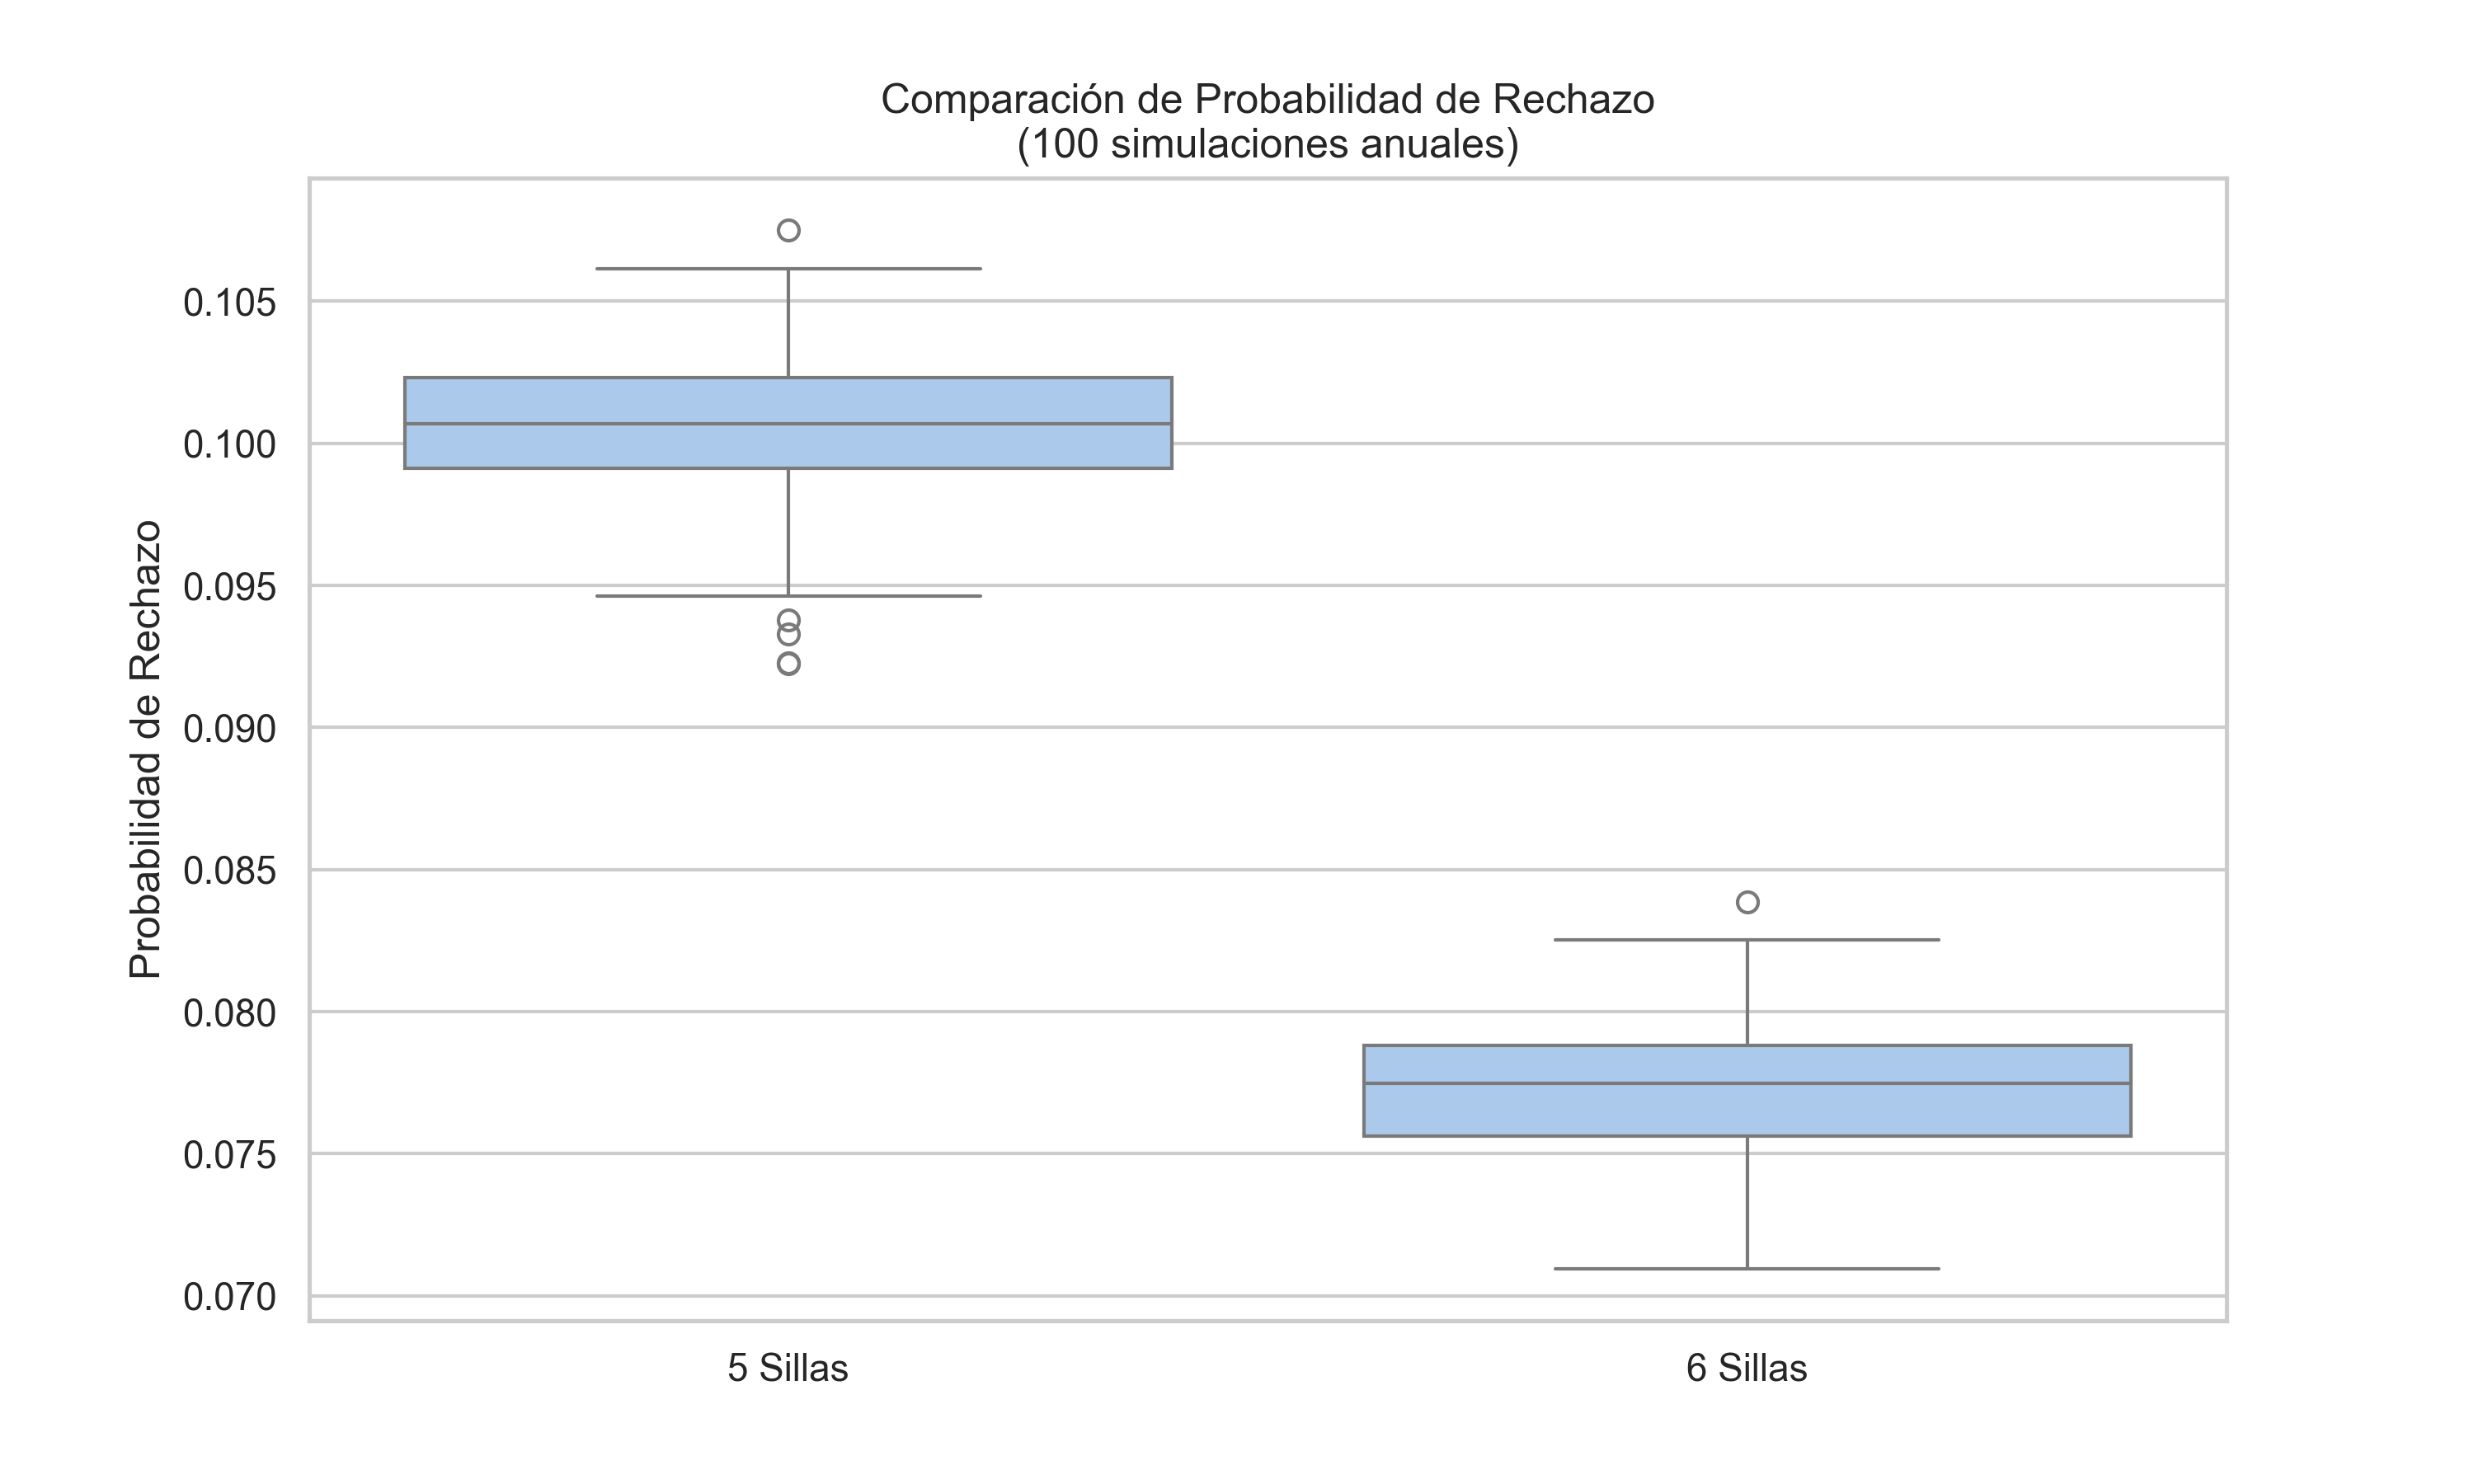
\includegraphics[width=0.75\textwidth]{../images/hipotesis_rechazo.png}
    \caption{Distribución de probabilidades de rechazo en ambas configuraciones. Se observa clara separación entre las distribuciones (solapamiento $<$ 0.1\%)}
    \label{fig:hipotesis}
\end{figure}

\textbf{Conclusión}: Rechazamos $H_0$ ($p < 0.05$). La diferencia es estadística y prácticamente significativa. La reducción promedio del 6.8\% implica que por cada 100 clientes:
\begin{itemize}
    \item Se perderían $\approx$10 clientes con 5 sillas
    \item Se perderían $\approx$3 clientes con 6 sillas
\end{itemize}
\section{Modelo Matemático}
El sistema se modela como una cola \textbf{M/M/1/5} con:
\begin{itemize}
    \item Tasa de llegada $\lambda = 5$ clientes/hora (Poisson)
    \item Tasa de servicio $\mu = 6$ clientes/hora (exponencial)
    \item Capacidad $k = 5$ clientes (1 en servicio + 4 en espera)
\end{itemize}

\subsection{Parámetros Clave}
\begin{align*}
    \rho &= \frac{\lambda}{\mu} = \frac{5}{6} \approx 0.8333 \\
    P_0 &= \frac{1 - \rho}{1 - \rho^{k+1}} = \frac{1 - 0.8333}{1 - 0.8333^6} \approx 0.1667
\end{align*}

\subsection{Probabilidades de Estado}
\[
P_n = P_0 \cdot \rho^n \quad \text{para } n = 0,1,\dots,5
\]

\begin{table}[H]
    \centering
    \caption{Probabilidades de estado estable}
    \begin{tabular}{cc}
        \toprule
        $n$ clientes & $P_n$ \\
        \midrule
        0 & 0.1667 \\
        1 & 0.1389 \\
        2 & 0.1157 \\
        3 & 0.0964 \\
        4 & 0.0804 \\
        5 & \textbf{0.0670} \\
        \bottomrule
    \end{tabular}
\end{table}

\subsection{Métricas Principales}
\begin{align*}
    L &= \frac{\rho}{1 - \rho} - \frac{(k+1)\rho^{k+1}}{1 - \rho^{k+1}} \approx 1.98 \text{ clientes} \\
    L_q &= L - (1 - P_0) \approx 1.15 \text{ clientes} \\
    P_{\text{rechazo}} &= P_5 \approx 6.7\% \\
    P(W > 0.75\text{h}) &\approx e^{-\mu t}\rho \approx 0.7\% \quad (t=45\text{ min})
\end{align*}

\section{Comparación con Simulación}
\begin{table}[H]
    \centering
    \caption{Resultados analíticos vs. simulación (1 año)}
    \begin{tabular}{lSS}
        \toprule
        Métrica & {Analítico} & {Simulación} \\
        \midrule
        $L$ & 1.98 & 1.9802 \\
        $L_q$ & 1.15 & 1.2305 \\
        $P_{\text{rechazo}}$ (\%) & 6.7 & 9.98 \\
        $P(W > 45\text{min})$ (\%) & 0.7 & 3.51 \\
        \bottomrule
    \end{tabular}
\end{table}

\section{Conclusiones}
\begin{itemize}
    \item La probabilidad de rechazo ($\approx$\SI{10}{\%}) sugiere que en horas pico se pierde 1 cliente cada 10.
    \item La espera $>$ 45 minutos es baja ($<$ 4\%), pero podría reducirse aumentando a 6 sillas:
    \[
    P_{\text{rechazo}}^{\text{(k=6)}} = \frac{(1-\rho)\rho^6}{1-\rho^{7}} \approx 3\%
    \]
\end{itemize}

\end{document}